\chapter{Testing with a classification tree}\label{sec:topic_5}

\section{Introduction}

If one wants to ensure that all possible cases are covered and checked in a test, the number of test cases can quickly become unmanageably large. If you have a certain number of parameters to consider in your tests, you have to try out and examine every possible combination of these tests to make absolutely sure that no unforeseen problem occurs. If parameters are also continuous, there is also the question of which intervals and values to consider. Depending on the resolution, this can be an unlimited number.

Classification trees (CT) offer an approach to reduce the complexity of such parameter constructions and to keep them clearly arranged. Test cases covering the relevant parameter constructions can then be derived from the CT. This chapter reviews the use of such CTs based on two selected articles describing their uses and suitability.

First, the literature search in the context of classification trees is explained. Subsequently, chapter \ref{Kap:Approach1} deals with classification trees as a method for creating test cases for model-based systems and discusses them. Using the movie manager as an example, the classification trees are applied to certain requirements. Chapter \ref{Kap:Approach2} then introduces Event Sequence Graphs (ESG) as an alternative concept for model-based systems. These are also applied to the movie manager example before a comparison of both approaches takes place in chapter \ref{Kap:Comparison}. Finally, a conclusion is drawn in chapter \ref{Kap:Conclusion}. There, we conclude by answering the question of the extent to which CT helped reducing a complex problem to a manageable number of test cases. As with the previous chapters, an attempt is then made to apply the design of this approach to the Movie Manager example.

\section{Literature search}

The literature search was conducted via snowballing and via a keyword search. Two partial approaches were used in snowballing. On the one hand, forward snowballing was used to find articles referencing the first given article. On the other hand, backward snowballing was used to search the articles that are listed by the initial article in the bibliography. Thus, publications directly related to the given article were considered. An overview of the main search results can be found in Figure \ref{fig:literature_search}. 

\begin{figure}[H]
\centering
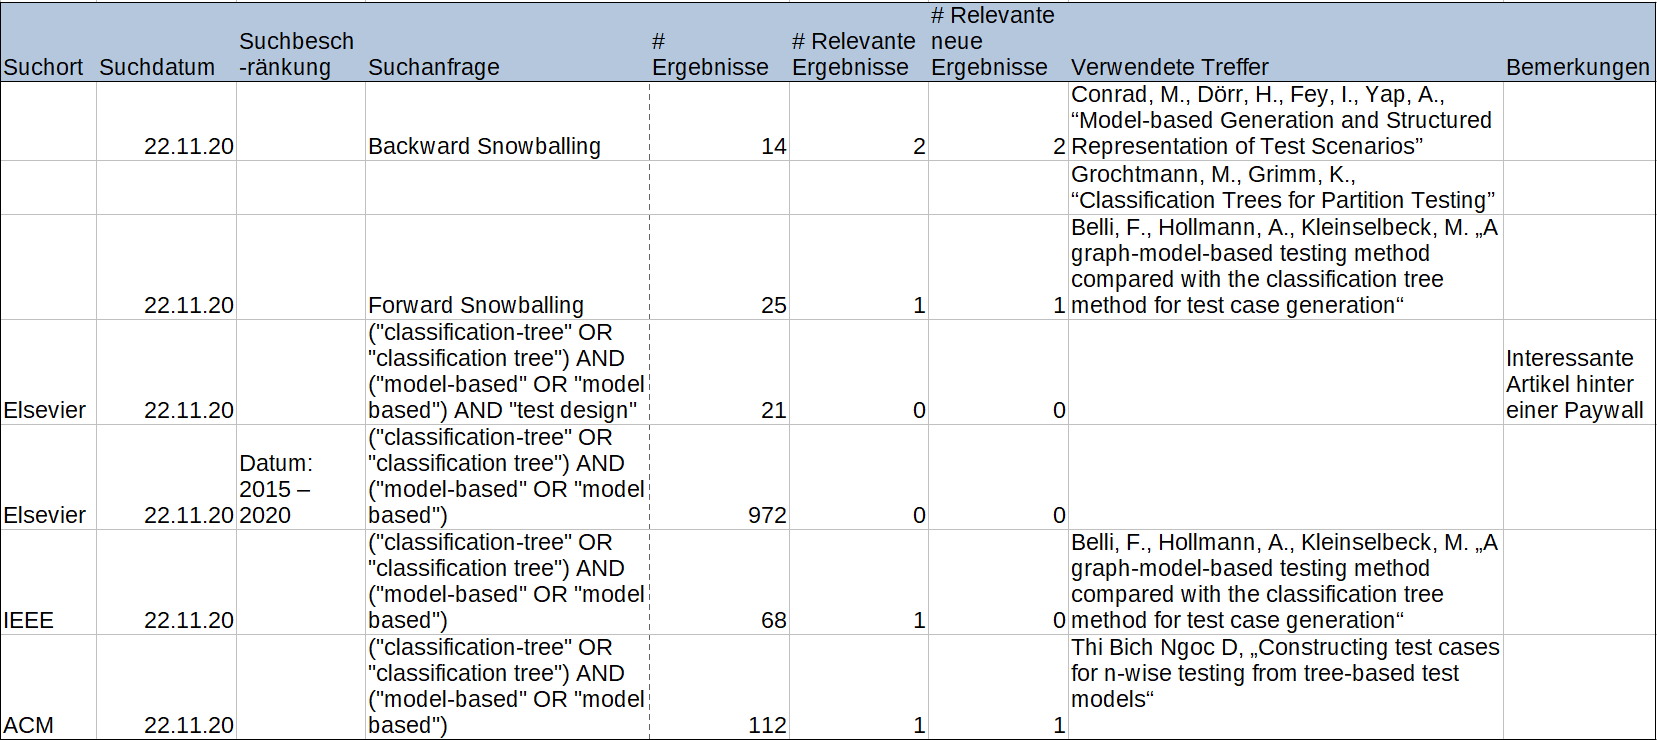
\includegraphics[scale=0.32]{../../individual/groeger/images/Suchdokumentation.png} 
\caption{The tabular documentation of the search. The relevant results are recorded on the basis of the parameters specified in the columns.}
\label{fig:literature_search}
\end{figure}

A free keyword search was then performed on Elsevier, IEEE, and ACM\footnote{Die Links zu diesen Suchmaschinen sind: Elsevier: https://www.sciencedirect.com/ IEEE: https://ieeexplore.ieee.org/Xplore/home.jsp ACM: https://dl.acm.org/ }. The search query reflects the exact wording that was finally used. During this process, experiments were conducted to estimate which keywords were relevant enough to elicit a suitable number of search hits. In addition, backward snowballing proceeded without experimentation by searching and evaluating the sources listed in the bibliography of the main article in order. Forward snowballing was performed by searching the citations given at Elsevier.

Figure \ref{fig:literature_search} shows the relevant results of both search approaches. The title and abstract of all results have been viewed, aside from the 1000 hits on Elsevier. There, the first fifty results have been considered. The assessment of whether an article is relevant was determined on the basis of three criteria:

\begin{enumerate}
\item CT must be used or described to allow conclusions to be drawn about their suitability
\item The article deals with testing or with the test design
\item The article must be available
\end{enumerate}

The first criterion is intended to filter out articles that do not deal with CT at all and thus do not allow any conclusions to be drawn. The second criterion is to filter out those documents that do not deal thematically with test cases or even software development. Often these articles deal with other types of \enquote{Classification Trees}. An example here are decision trees or graphical visualizations of the classification of objects in artificial intelligence. These trees describe other phenomena or  other problems. However, this chapter is explicitly about the use of such trees for the generation of test cases.

Both approaches to the search yielded multiple hits. One of the articles listed among the relevant search results occurred in the search using both approaches, giving it additional relevance to the topic. Accordingly, the article \enquote{A Graph-Model-Based Testing Method. Compared with the Classification Tree Method for Test Case Generation} by Belli and Hollmann\cite{Belli} has been selected.

\pagebreak

\section{Approach 1: Systematic Model-Based Testing of embedded automotive software}
\label{Kap:Approach1}

\subsection{Description}

The first approach comes from Conrad et al\cite{Conrad}: The article \enquote{Systematic Model-Based Testing of Embedded Automotive Software} deals with the application of CT to problems that have a simulation or model of the application. The application example of the paper is the testing of an ABS system. Therefore, the introduction starts with a comparison of traditional and model-based software development. Figure \ref{fig:tradditional_vs_modelbased} from the article shows this difference well. The necessity of model-based test methods is thereby justified. The approach introduced as \enquote{model-based black-box testing} (MBBBT) is presented below. Two perspectives are presented: Requirements-based test design and model-based test design. The basis for this is the creation of a CT.

\begin{figure}[H]
\centering
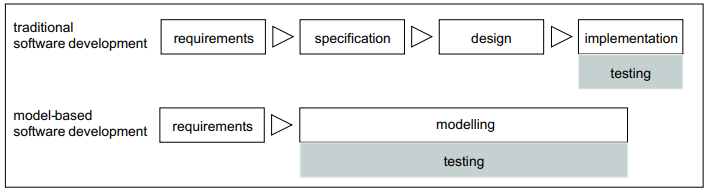
\includegraphics[scale=0.75]{../../individual/groeger/images/TraditionalVSModel.png} 
\caption{This figure shows the difference between traditional development and model based developement. This article examines CT for projects with a model of the application. \cite{Conrad}}
\label{fig:tradditional_vs_modelbased}
\end{figure}


A graphically represented CT consists of the following components: The root denotes the product or model. The branches derived from it define the classifications. Classifications describe different requirements of the product. This depends on which of the two perspectives mentioned above was chosen as the basis. The leaves of a CT describe the different classes. A class in this context is a qualitative description. Thus, a category is described by the classes here. We can also say the range of values of a category is decomposed into the different classes. Figure \ref{fig:ABS_CT} shows the requirements-based CT for the ABS model. At the top of the figure are the individual classifications with the different values for the classes. Because this is a requirements-based CT, mostly qualitative descriptions such as \enquote{dry}, \enquote{straight}, or \enquote{strong braking} are found as leaves.  

For the test cases, the combination of these leaves is now to be tested. If you test all combinations of classes of this CT, you cover all test cases defined via the requirements. This assumes that the requirements are complete. In this example, this results in $4*2*3*5 = 120$ combinations.

The next step is the generation of a CT more suitable for the actual model that is used in the developement. Classification now describe different parameters. Classes contain quantitative value or an interval for the input parameters of the model. 

\begin{figure}[H]
\centering
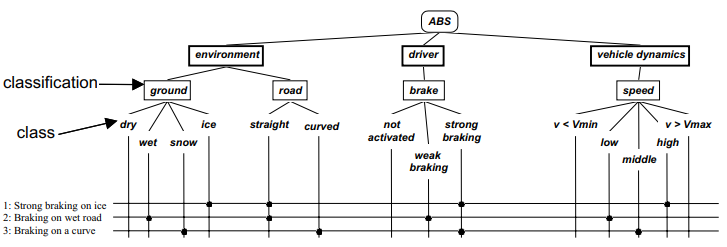
\includegraphics[scale=0.75]{../../individual/groeger/images/ClassificationTreeExample.png} 
\caption{This figure shows the CT made for the use case. The top part shows the different classifications and classes of the tree while the lower part shows the construction of test cases from the combination of leaf nodes.}
\label{fig:ABS_CT}
\end{figure}

Thus, for both perspectives, a CT is created and compared to analyze whether the requirements are covered by the model-based test scenarios. In this process, the classes of the requirements tree are mapped to the model tree. A model-based tree, on the other hand, describes the input dimensions or model parameters. Qualitative descriptions must therefore be transformed into the input parameters of the model. \cite{Conrad} discusses 1:1 and 1:n relations. 1:1 relations represent unique mappings, while 1:n reflects an occurrence of the corresponding requirement class in multiple parameters of the model. If this mapping is successful, a requirement class can be covered by testing the related classes in the model tree. The relations of the example classes of the ABS are summarized in a table for both trees. The summary explains the advantages of the MBBBT despite higher expenditure by the classification of two different approaches and recommends the application of this approach with the software development with models.

\subsection{Application}

The approach of a CT requires as a basis a model, over which is tested and after the approach of \cite{Conrad} also requirements, which can be mapped on it. Test cases are then determined from this by combining the classes and tested over the model. In this example, there is no real, simulatable model to describe it, but there is a description of requirements that could be mapped into a CT. The requirements described are:

\begin{enumerate}
\item film	
	\begin{enumerate}
		\item A movie must be able to be added including description.
		\item A movie must be able to be removed
	\end{enumerate}
\item actor
	\begin{enumerate}
		\item It must be possible to describe a performer
		\item A performer must be able to be linked to a movie
		\item An actor must be able to be removed
	\end{enumerate}
\item Previous movies
	\begin{enumerate}
		\item Previous movies must be saved
	\end{enumerate}
\item rating
	\begin{enumerate}
		\item It must be possible to rate a movie
		\item It must be possible to display the rating of a movie
	\end{enumerate}
\end{enumerate}

\begin{figure}[H]
\centering
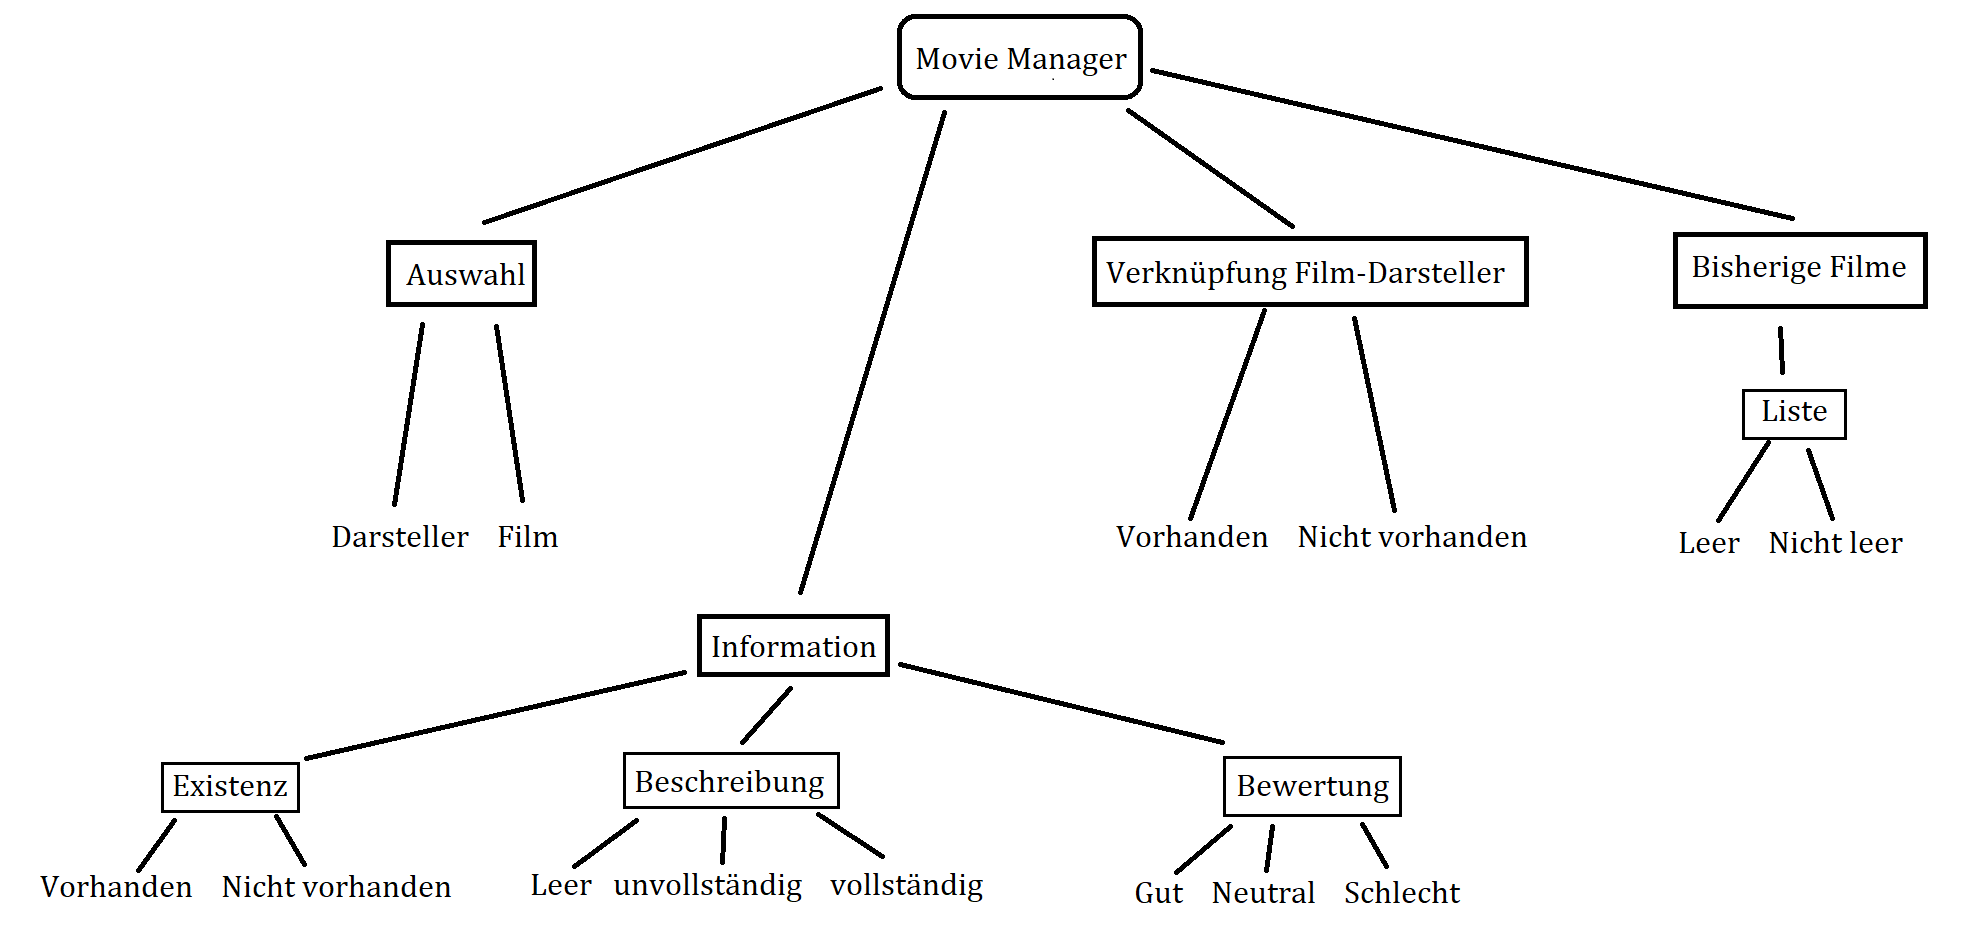
\includegraphics[scale=0.25]{../../individual/groeger/images/Anforderunsbaum.png} 
\caption{The requirements-based CT for the Movie Maker example defines the various classifications and classes for the test cases. Only a transformation into model parameters has to be done before the test cases can be constructed.}
\label{fig:Movie_Maker_CT}
\end{figure}

The requirements presented here can then be transformed into a requirements-based CT as in Figure \ref{fig:Movie_Maker_CT}. In the absence of a proper model against which to make classifications, exactly what counts as input or class depends on the exact implementation. A possible transition to \cite{Conrad} can be found in the following illustration: The requirements shown here can then be transitioned to a requirements-based CT as in Figure \ref{fig:Movie_Maker_CT}. In the absence of a proper model against which to make classifications, exactly what counts as input or class depends on the exact implementation. A possible transfer to \cite{Conrad} can be found in the following illustration:

\begin{table}[t] 
\centering
\begin{small}
\caption{A tabular listing of the various requirements with example values. The last column indicates which type of transfer is possible with a suitable implementation.}
\label{tab:ueberfuehrung}

\setlength{\tabcolsep}{1em}
\begin{tabular}{ p{2.4cm}| p{3cm} |p{5cm} |p{1.3cm} }
	\hline
	\textbf{Klassifizierung} & \textbf{Klasse} & \textbf{Modellwerte} & \textbf{Relation} \\
	\hline	
	Auswahl & Darsteller & Object: Darsteller & 1:1 \\
	\hline
	   & Film & Object: Film & 1:1 \\
	\hline
	Existenz & Vorhanden & Valid & 1:1 \\
	\hline
	   & Nicht vorhanden & NULL & 1:1 \\
	\hline
	Beschreibung & Leer & [\enquote{}] & 1:1 \\
	\hline
	   & Unvollständig & [\enquote{Name}:\enquote{x}] & 1:n \\
	\hline
	   & Vollständig & [\enquote{Name}:\enquote{x}, \enquote{Veröffentlichung}:\enquote{20XX}, ...] & 1:n \\
	\hline
	Bewertung & Gut & [ 5.0, 3.0 ] & 1:1 \\
	\hline
	   & Neutral & ] 3.0, 2.0 [ & 1:1 \\
	\hline 
	   & Gut & [ 5.0, 3.0 ] & 1:1 \\
	\hline 
	Verknüpfung & Vorhanden & [\enquote{Darsteller}:\enquote{Max Mustermann}, \enquote{Film}:\enquote{XY}] & 1:n \\
	\hline 
	   & Nicht vorhanden & NULL & 1:1 \\
	\hline 
	Bisherige Filme & Leer & NULL & 1:1 \\
	\hline 
	   & Nicht leer & [\enquote{Film}:\enquote{XY}], [\enquote{Film}:\enquote{X}, \enquote{Film}:\enquote{Y}, ...] & 1:n \\
	\hline 
\end{tabular}
\end{small}
\end{table}

Based on this transfer, it is then possible to determine suitable test cases. This results from the combinations of the different classes. Assuming that n is only 1 for the 1:n relations, the classifications for selection, existence, description, evaluation, linkage and the previous films result in $2*2*3*3*2*2 = 144$ combinations of test cases. Individual test cases can then be, for example, the following:

\begin{itemize}
\item Entry of a movie that already exists but has an incomplete description (Selection: Movie, Existence: Existing, Description: Incomplete, etc.)
\item Linking an actor to a non-existing movie (Selection: Actor, Existence: Nonexistent,Link: Nonexistent, etc.).
\item Add a movie to an empty list of already viewed movies (Selection: Movie, Existence: Existing, Previous movies: Empty, etc. )
\end{itemize}

These are individual test cases. If you work through all combinations, the tests are considered complete. In some cases, its not necessary to test ALL combinations, since some combinations may not be possible or distinctive. Testing the first example in the list above is independend from the rating of the movie. But testing all combinations ensures that all parameters have been checked, assuming the classification tree is complete.

\section{Approach 2: A Graph-Model-Based Testing Method compared with the Classification Tree Method for Test Case Generation}
\label{Kap:Approach2}

\subsection{Description}

The selected article \enquote{A Graph-Model-Based Testing Method Compared with the Classification Tree Method for Test Case Generation} starts with a description of the difficulties and complexity of testing under time pressure. Quickly, a newer method, \enquote{Event Sequence Graphs} (ESG), is introduced in addition to CT in the context of electronic control unit development. The next chapter explains some basics for this. Besides an explanation of CT, this section also contains a formal description of ESG. Here, a graph with its nodes represents events, including start and end events. Start nodes are the user inputs and end nodes are the final system responses. the graph thus contains valid system flows while the complementary graph contains invalid system flows. The article describes valid tests as those that successfully traverse an ESG from start to finish or successfully cause the flows of the complementary graph to fail.

\begin{figure}[H]
\centering
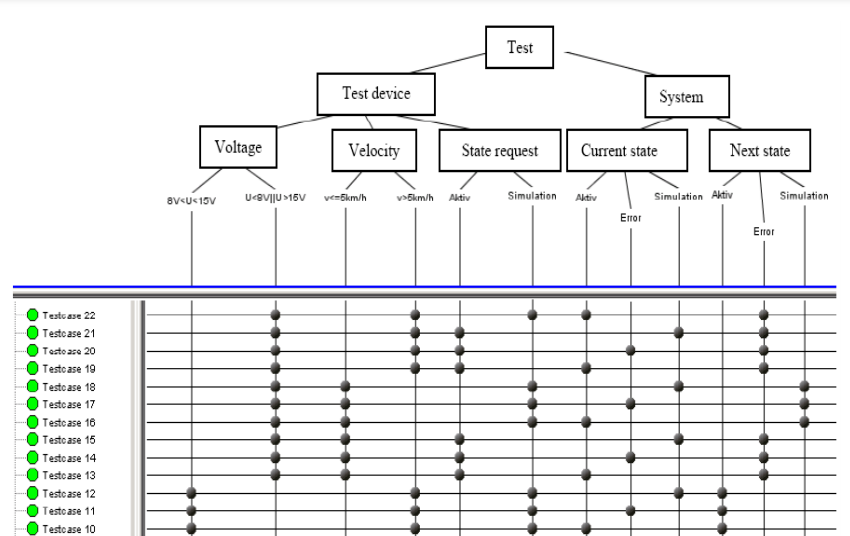
\includegraphics[scale=0.6]{../../individual/groeger/images/ClassificationTreeExample2.png} 
\caption{This is the CT for the second approach. A requirements-based perspective is dispensed with. Instead, the focus is on comparison with ESG.}
\label{fig:Approach2_CT}
\end{figure}

While CTs look at different combinations of input values, ESGs look at combinations of different sequences of inputs. They then evaluate whether this sequence of \enquote{events} resulted in a success or failure of the action and whether that was part of the expected behavior. Unlike CT, which only looks at what should work, ESGs thus also consider failures.

Then, after the formal description, the test scenario is presented: A control system with ABS, ESP and an adaptive control element. This is followed by a description with specific characteristics of the test environment. The study starts with the application of ESG and CT to the previously described test environment. Difficulties with CT are mentioned, citing dependencies that are difficult to understand. As a result of the study, a lower effort for the creation of CT test, but also a higher number of test cases and thus test steps are mentioned. Both approaches uncovered approximately the same errors. Figure \ref{fig:Comparison_CG_ESG} shows the main findings of the comparison from Belli and Hollmann's\cite{Belli}'s test study.

\begin{figure}[H]
\centering
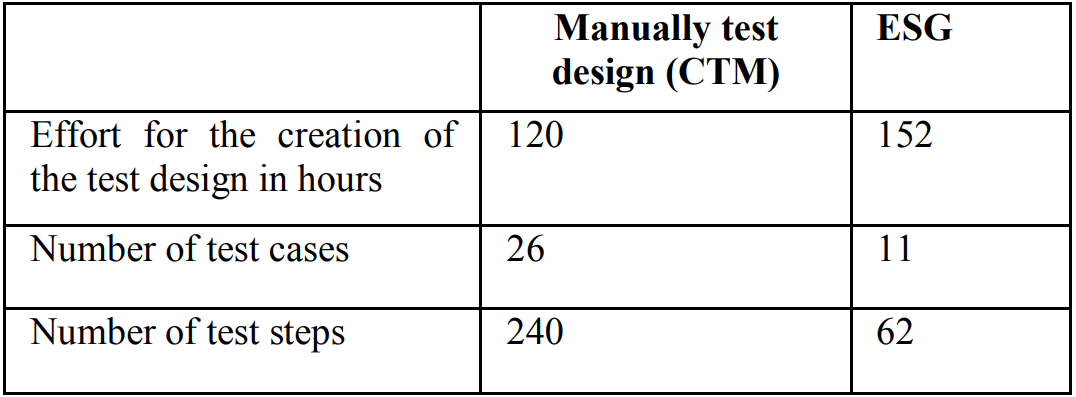
\includegraphics[scale=0.4]{../../individual/groeger/images/Comparison_CG_ESG.png} 
\caption{This table shows the results of the comparison between CT and ESG.}
\label{fig:Comparison_CG_ESG}
\end{figure}

The table shows that CT and ESG offer their advantages and disadvantages. The effort required for test design is slightly higher for ESGs, while ESGs perform better in terms of the number of test cases and test steps. This shows that CT can at least keep up with ESG in comparison.

\subsection{Application}

The CT, as they are built and used here, are identical in their function. In the article, a model-based CT is built directly without looking at the requirements themselves. This makes it all the more necessary to have a model for simulation or a ready-made application environment. Nevertheless, the same table as in Figure \ref{fig:Approach1_CT} would arise at this point.

Regarding the ESG, similar difficulties appear when trying to adapt this model based approach to the move manager example. Figure \ref{fig:ESG_example} shows an example for a partially constructed ESG. Test cases can be constructed by triggering events with Inputs or user actions. Test cases are successful, if they reach the exit event on the right side. Such a test could be: 

\begin{enumerate}
	\item Starting with an \enquote{empty data base}
	\item Adding a movie, reaching \enquote{movie exists}
	\item Adding a performer, reaching \enquote{Movie and performer exist}
	\item Linking movie and performer
	\item Closing the application without and error, leading to the exit event.
\end{enumerate}

\begin{figure}[H]
\centering
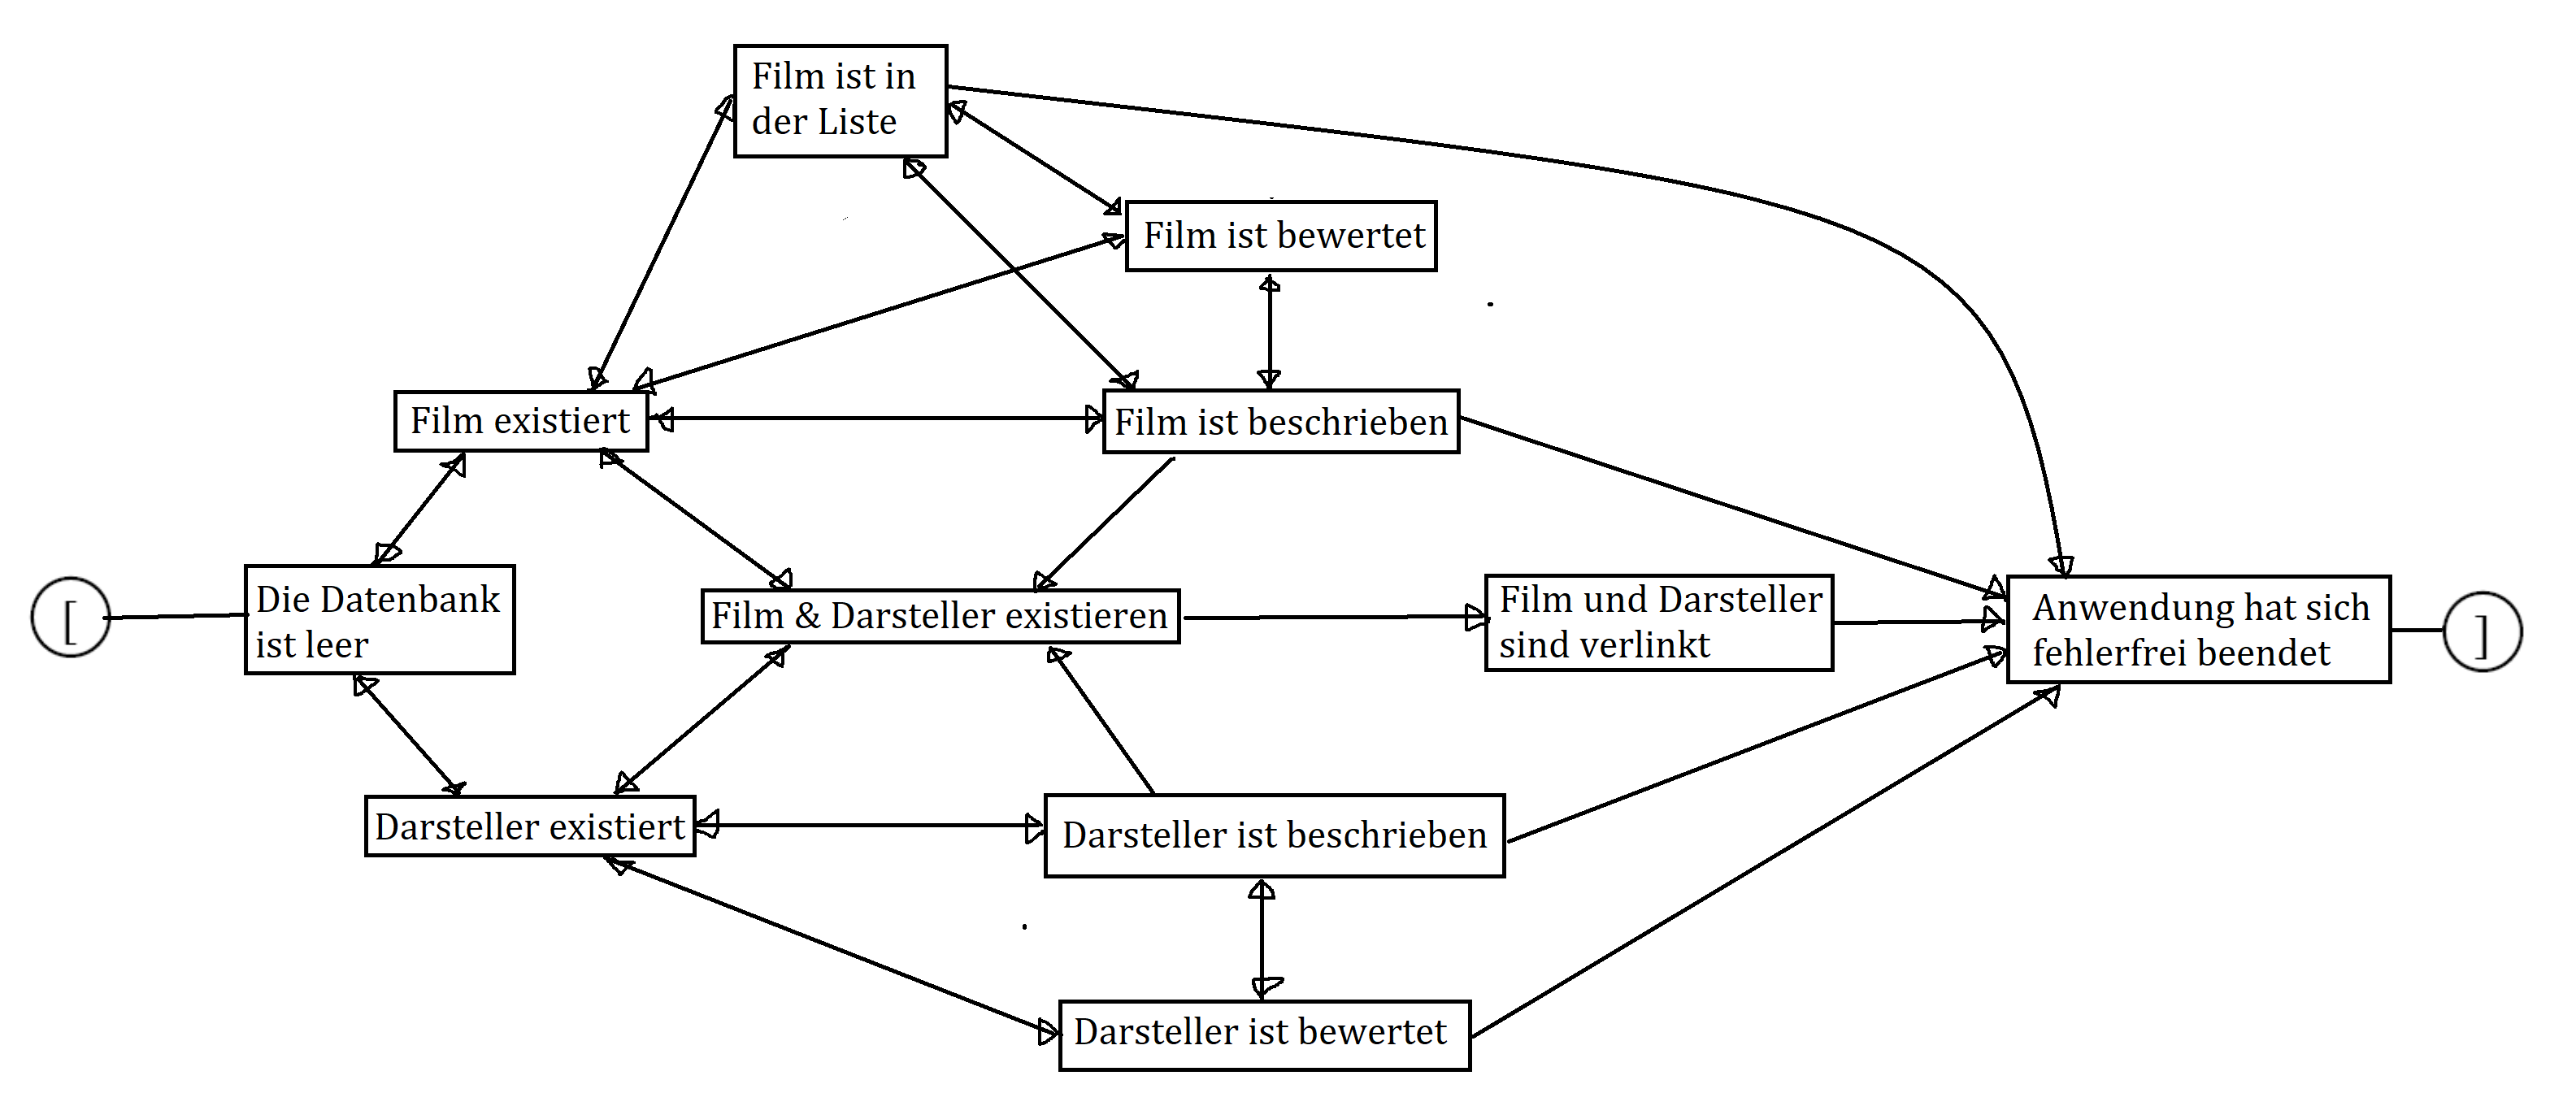
\includegraphics[scale=0.175]{../../individual/groeger/images/ESGamBeispiel.png} 
\caption{An example for possible event sequences to construct test cases.}
\label{fig:ESG_example}
\end{figure}

\section{Comparison}
\label{Kap:Comparison}

\begin{small} 		
	\begin{longtable}[h]{p{0.45cm}|p{0.425\textwidth}|p{0.425\textwidth}}
	\caption{The synthesis matrix summarizes the differences, similarities and peculiarities that stood out during the synthesis.}
	\label{tab:synthesematrix_julian}
	\\    %%%%<===
	\hline
	\textbf{Nr.} & \textbf{Conrad and Fey} & \textbf{Belli et al.} \\
	\hline
	1a) & Anforderungsbasierte CT, Modellbasierte CT,  1:1 und 1:n Relationen & CT, ESG, tabellarischer Vergleich \\
	\hline	
	1b) & Simulierbares Modell liegt vor, Anforderungen können im Modell abgebilded werden & Simulierbares Modell liegt vor \\
	\hline	
	1c) & 1. Entwurf zweier CT für Anforderungen und Modell. 2. Abbildung Anforderungen -> Modell 3. Testentwurf durch Kombination aller Klassen & 1. Entwurf CT und ESG 2. Testentwurf durch Kombination aller Klassen / Zustandsübergänge 3. Vergleich in Tabelle \\
	\hline	
	2a) & Testentwurf mit (black box)-Modellen & Testentwurf mit (black box)-Modellen \\
	\hline	
	2b) & Softwareentwickler & Softwareentwickler \\
	\hline	
	2c) & Software Testing, Software Maintenance and Software Construction & Software Testing, Software Maintenance \\
	\hline
	3a) & Matlab Simulink & CANoe \\
	\hline
	3b) & 1. Manuell , 2. Manuell , 3. Automatisierbar & 1. Manuell, 2. Vollatomatisierbar, 3. Manuell \\
	\hline	
	4a) & Vergleich der Klassifikationsbäume & 
	Vergleich der Teststatistiken  \\
	\hline	
	4b) & Sehr gut geeignet für black box Modelle auf Basis von Anforderungen & CT sind ein guter Ansatz neben ESG. CT sind schneller zu entwickeln, aber haben größere Tests \\
	\hline	
	\end{longtable}
\end{small}


\newpage
\paragraph{Focus}

In \cite{Conrad}, the special feature is the mapping from requirements-based CT to model-based CT. This is used to ensure that requirements are met by testing a model. From this, a procedure can be derived to formulate a CT from the requirements and apply it to the input parameters of its model or product. In the end, the use of CT for problems with models is recommended. 

In \cite{Belli}, the main focus is the integration of ESG and its comparison with the application of a CT. With this, advantages and disadvantages with related methods can be determined.

\paragraph{Commonalities}

Both approaches deal with the application of CT to model-based test designs. As a result, the prerequisites are similar. The supported usage scenarios and stakeholders are also the same. This is mainly due to the fact that both approaches primarily target an application within the automotive industry. The level of automation is similar in that the test design seems harder to automate due to the level of abstraction.

\paragraph{Differences}

With its focus on the ESG, \cite{Belli} clearly differentiates itself from \cite{Conrad}. As a result, the evaluation also focuses on comparison, while \cite{Conrad} focuses more on usability. Different tools and programs were also used to reach the goal. \cite{Conrad} also goes more intensively into the CT. This is recognizable by the fact that the determination of a CT is dealt with in more detail via a transfer of the requirements.

ESG itself is distinguished from CT, as described in the previous chapters, by considering a combination of possible state and input sequences instead of a combination of possible input values, which also makes it possible to ensure that cases that should not work do not work.

Figure \ref{tab:synthesematrix_julian} shows the synthesis matrix of the two articles on which the comparison of this chapter is based. 

\section{Conclusion}
\label{Kap:Conclusion}

The search on snowballing is promising and also offered relatively many relevant articles. With a free search, the risk of being flooded with irrelevant hits is greater. This makes sense in that snowballing exploits a direct link via the citations, and free search does not require articles to be related. Thus, articles about decision trees or about testing thematically inappropriate use cases such as medical procedures also appeared among the results. In contrast, one has a wider reach, provided one chooses the search terms appropriately.

Classification Trees offer the possibility to reduce the number of test cases. It turns out that CT are well suited for model-based problems, but it can be difficult to represent arbitrary tasks in this way.  \cite{Conrad} shows for this case how to transform requirements into a CT for the input parameters of a system model. However, the existence of a model-like description remains necessary. According to \cite{Belli}, it is shown that CTs nevertheless remain relevant, even alongside more recent methods.








